\documentclass[12pt, letterpaper]{article}
\usepackage[utf8]{inputenc}
\usepackage{graphicx}
\usepackage{hyperref}
\usepackage{fancyvrb}
\usepackage{array}
\usepackage{biblatex}
\usepackage{float}
\usepackage{subcaption}

\bibliography{rapport}

\title{Fiche de lecture : Réseau neuronal convolutif}
\author{Chaolei Cai
\\
    \multicolumn{1}{
        p{.7\textwidth}}{\centering\emph{Université Paris Vincennes St-Denis\\
  UFR mathématiques, informatique, technologies sciences de l'information\\}
  L3 Informatique}
}
\date{\today}
\begin{document}


\begin{titlepage}
    \maketitle
\end{titlepage}

\tableofcontents

\section{Avant-propos}
Ce document est ma fiche de lecture sur le réseau neuronal convolutif (Convolutional Neural Network or ConvNet), il fait partie de la notation pour 
le cours de programmation pour l'intelligence artificiel enseigné par M.Jean-Jacques Mariage aux L3 de la licence informatique.\\
Dans le plan géneral, je vais vous présenter le néocognitron, un ancêtre des CNN.\\
Dans un second temps, je vais m'intéresser à une publication d'Alex \\Krizhevsky, Ilya Sutskever et Geoffrey E.Hinton sur la classfication d'image via un Deep Convolutional Neural Networks.\\
Enfin je terminerai sur un article de Amir Rosenfeld, Richard Zemel et John K. Tsotsos qui pointe les limites rencontrées par les modèles CNN les plus moderne.

\section{Néocognitron}
\subsection{Présentation de l'auteur}
M.Fukushima est un chercheur en informatique connue pour ses travaux dans le domaine du réseau de neuronne artificiel et du deep learning.
Le plus célèbre étant son modèle de Néocognitron publié en 1980 \autocite{Fukushima:1}.

\subsection{Présentation de l'article}
Le néocognitron est un modèle élaboré depuis le modèle de cognitron publié par le même auteur en 1975. 
Il s'agit d'un réseau de neuronne multi-couche auto-organisatrice. L'apprentissage n'est pas supervisée, c'est à dire que 
les données ne sont pas étiquetées. Il s'inspire notamment des travaux de Hubel et Wiesel sur le système visuel animal (chat).
\autocite{HubelWiesel:2}. A nos jour, la recherche a bien évidemment avancé depuis 1959, Le model d'Hubel et Wiesel n'est plus tout à fait exacte 
mais reste intéressant dans les grandes lignes. Un des professeur en physiologie m'avait d'ailleurs présenté ces travaux quand j'étudiais encore à la 
licence Science pour la santé à Paris Descartes quelques années auparavant. \\
Le point important à retenir c'est que Hubel et Wiesel propose l'idée qu'un réseau de neuronne 
reste quand même traditionnel.\\
 neuronne est 
constitué de cellule "Simple" appelée "S-cells" et de cellule "Complex" appelée "C-cells".\\
Pour être tout à fait précis, le neocognitron ne reconnais pas l'object complexe mais présente plutôt un 
capacité à reconnaitre des patternes de stimuli précis après l'entraînement.\\
Notre sujet présente une organisation étalé sur plusieurs couche, dans l'idée, il faut retenir qu'il s'agit d'un réseau organisé neuronne 
reste quand même traditionnel.\\
 en cascade et hierarchisé.

\subsection{Présentation de la structure}
Au niveau de l'entrée, nous pouvons trouver des cellules photoreceptrices chargées de transmettre l'information. Si nous devons faire un rapprochement avec le réel, cela correspond aux rétines sensible à différentes stimulis lumineuse.\\
Dans la suite intervient une succession de module, une module est constitué d'une ou plusieurs couche de neuronnes.
La première constituée de cellules simples, l'auteur appelle cette couche "S-layer", puis arrive les couches complexes constituées 
à leur tour de cellules complexe voire hyper-complexe, de la même manière, ils portent le nom de "C-layer".
Il est intéressant de noter que seul les synapses partant vers une "S-cell" ont la propriété de plasticité. La plasticité en neuroscience 
est le terme pour désigner le capacité d'un neuronne à former et modifier ses connexions vers d'autre neuronne via les synapses. 

\begin{figure}[H]
    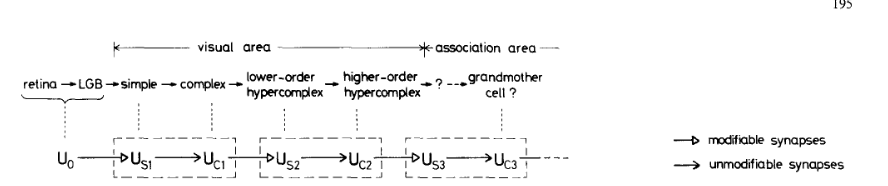
\includegraphics[width=\linewidth]{img/fig1.png}
    \caption{Correspondence between the hierarchy model by Hubel and Wiesel, and the neural network of the neocognitron}
    \label{fig:L1}
\end{figure}

Comme vous pouvez le voir sur ce schéma, U0 est notre couche d'entrée, par la suite intervient une cascade de module constitué par différentes couches de cellules.
Au sein d'une même module, les liens entre les neuronnes de différentes couches sont fixes, alors qu'à la jointure des 
modules, ces liens sont modifiables et peuvent être amènés à évoluer au fur et à mesure de l'apprentissage.
Tout cela nous permet de faire un parallèle avec le fonctionnement du cortex visuel et associatif.
\begin{figure}[H]
    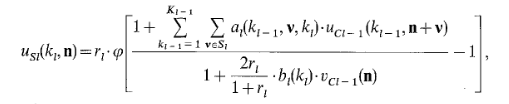
\includegraphics[width=\linewidth]{img/fig2.png}
    \caption{formule de la sortie d'une cellule S}
    \label{fig:L2}
\end{figure}
D'après cette formule, la sortie d'une cellue S situé à la couche k d'un module l de notre réseau dépends essentiellement 
de $al(k(l-1), v, kl)$ et de $bl(kl)$ qui correspondent à l'efficacité des synapses exitatoire et inibitoire.\\
Il est possible de rendre la cellule plus ou moins sélective à une patterne d'excitation en variant $rl$. \\
En ce qui concerne le mécanisme d'auto-organisation, à chaque fois qu'une entrée arrive, des "S-cell" répresentatives sont selectionnées, et vont 
voir renforcé leur synapses d'entrée. Au contraire ceux qui ne manifeste aucun sensibilité ne sont pas renforcé. Au fur et à mesure de l'apprentissage, 
nous verrons alors apparaître sur le plan cellulaire des colonnes, une succession de zone qui sont sensible à un même stimulis sur différente couche.
\begin{figure}[H]
    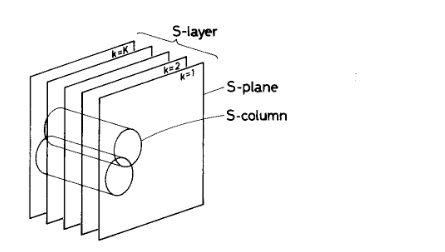
\includegraphics[width=\linewidth]{img/fig3.png}
    \caption{Relation between S-planes and S-columns within an S-laye}
    \label{fig:L3}
\end{figure}

Ainsi, nous construisons un réseau qui dans les première niveau de profondeur ne va que reconnaitre des patterne simple et élementaire, et plus nous progressons 
dans le réseau, les éléments basic se regroupe en motifs, jusqu'à l'obtention d'un "objet".\\
Comme le schéma ci-dessous le montre, il y a la reconnaissance de trait basique puis dans les niveaux plus profondes, le motif de la lettre 'A' est 
reconstruite. \\
Ici, la connexion n'est pas total entre les différentes couche, il y a donc beaucoup moins d'information à traîter et la structure est plus légère.
Au final, le réseau n'est pas si chargé, car les "S-columns" peuvent parfaitement s'entre croiser. Il est tout à fait possible que pour la lettre 
'R' et 'B' partagent les même cellules comme ces 2 lettres sont proche au niveau de l'écriture. \\
Enfin, notre réseau offre une tolérance vis à vis des déformations, changement d'orientation et changement de position car quelque soit 
l'entrée présenté, il est divisé en sous composante puis reconstruite dans les profondeur.
Nous pouvons déja voir ici les prémices du CNN, nous pouvons aussi remarquer que le réseau est neuronne 
reste quand même traditionnel.\\
 à sens unique, 
sur les schémas ci-dessous par exemple, l'information va toujours de la gauche vers la droite, il n'y a qu'un seul mouvement, celui de feedfoward. \\
Alors que sur les modèles CNN moderne, nous pouvons trouver une étape de backpropagation.

\begin{figure}[H]
    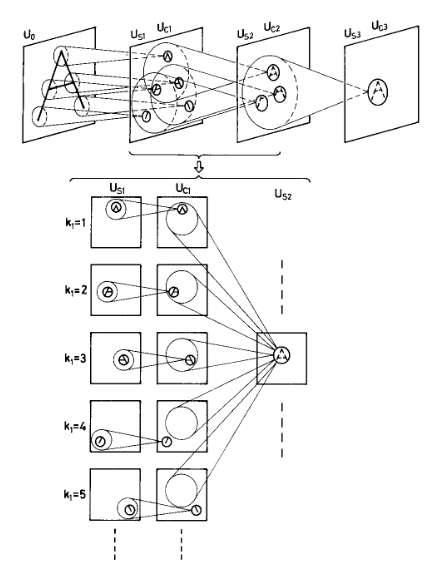
\includegraphics[width=\linewidth]{img/fig4.png}
    \caption{An example of the interconnections between ceils and the response of the cells after completion of self-organization}
    \label{fig:L4}
\end{figure}

\begin{figure}[H]
    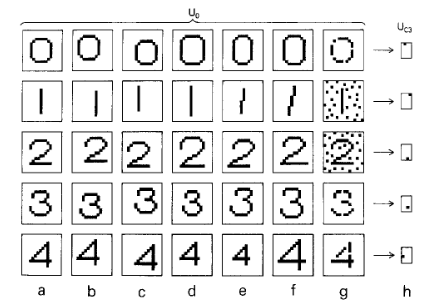
\includegraphics[width=\linewidth]{img/fig5.png}
    \caption{Some examples of distorted  stimulus patterns  which the neocognitron has correctly recognized, and the response of the final layer of the network }
    \label{fig:L5}
\end{figure}
\begin{figure}[H]
    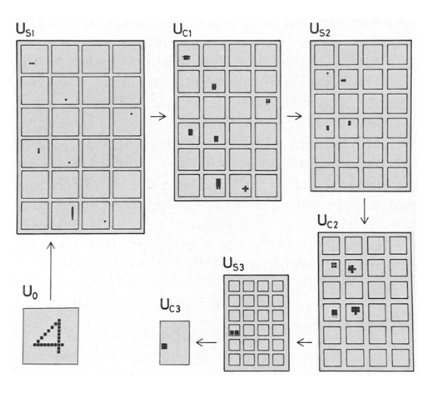
\includegraphics[width=\linewidth]{img/fig6.png}
    \caption{A display of an  example of the response of all the individual cells in the neocognitron}
    \label{fig:L6}
\end{figure}

\section{Réseau neuronal convolutif}
\subsection{Présentation des auteurs}
Alex Krizhevsky, Ilya Sutskever et Geoffrey E. Hinton étaient des étudiants de l'université de toronto au moment de la publication 
de cette article \autocite{NIPS2012_4824:3}, J'ai préferé cette article plutôt qu'un des nombreuses publication de M.Yann Lecun car au niveau 
du contenue cette article est plus simple à comprendre au niveau de la lecture.
Le premier auteur travail maintenant chez Google, les 2 autres continuent à publier régulièrement des article jusqu'à ce jour.

\subsection{Présentation l'article}
\par Ce n'est pas eux qui inventent le CNN mais il est interessant de noter le bond gigantesque au niveau des performances des CNN sur ImageNet après 2012.
Notamment pour la compétition ILSVRC-2012 les auteurs ont réalisé une performances de 15.3\% taux d'erreur alors que le second 
du concours n'arrivait qu'à 26.2\%.\\
L'article est populairement cité dans le domaine, google indique d'ailleurs que le nombre de citation dépasse les 60k.
Le dataset utilisé ici est celui d'ImageNet qui est constitué à peu près de 15 millions d'image dans plus de 22 milles catégories.
A l'opposé, le MNIST dataset de M.Yann Lecun ne contient que 60k exemples, évidemment il faut prendre en compte que la complexité 
de l'information n'est pas pareil quand vous comparer des chiffres manuscrites et des images d'objet réel.
Le progrès majeur apporté par cet article est qu'il s'agit d'une implémentation GPU de Deep CNN, La structure de leur réseau de neuronne 
reste quand même traditionnel.
\par L'avantage majeur du CNN est qu'il ne nécessite pas une connexion total entre les couches, il y a donc moins de paramètre et de poids à ajuster lors
de l'apprentissage. Malgré ces qualités, le CNN reste gourmands en terme de mémoire et en performances car le produit de convolution est coûteuse à calculer.
D'où l'implémentation sur le plateforme GPU, accompagné d'optimisations accrues pour le produit de convolution 2D. \\
Le système prends en entrée une image RGB de dimension 256x256, une réadaptation de l'image a été effectué pour avoir des "patch" de dimension valide.


\subsection{Présentation de la structure}
\begin{figure}[H]
    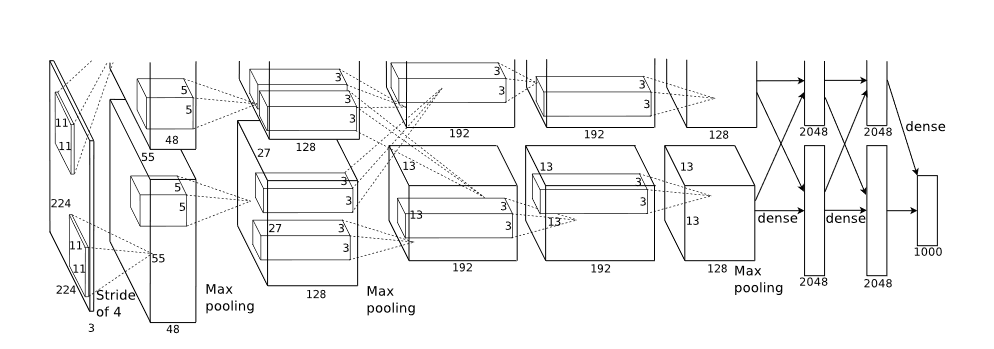
\includegraphics[width=\linewidth]{img/fig7.png}
    \caption{An illustration of the architecture of our CNN, explicitly showing the delineation of responsibilitiesbetween the two GPUs. One GPU runs the layer-parts at the top of the figure while the other runs the layer-partsat the bottom. The GPUs communicate only at certain layers. The network’s input is 150,528-dimensional, andthe number of neurons in the network’s remaining layers is given by 253,440–186,624–64,896–64,896–43,264–4096–4096–1000.}
    \label{fig:L7}
\end{figure}
Comme le montre le schéma ci-dessus le montre, le réseau de neuronne est constitué de 5 couches de convolution puis de 3 couches "fully-connected".
2 Cartes graphiques sont nécessaire pour cet implémentation, chaque carte traîte ses couches à lui, une communication entre les 2 cartes graphiques n'est 
possible qu'à une certaine couche précis.
\par Le coeur du CNN est le produit de convolution, donnant une image d'entrée de dimension $a*b$, la première couche de convolution va y passer et produire 
à son tour plusieurs sous image qui seras plus petite à cause du filtre. Au fur et à mesure des calcules, plus vous avancer dans la profondeur du réseau, plus les neuronnes seront petit, 
à la fin vous obtiendrez une sorte de carte 2d constitué de neuronne. Ces derniers auront une réponse spécifique à un stimulis précis.
\par La manière standard de corriger la sortie d'un neuronne est d'utiliser une fonction $f(x) = tanh(x)$ ou encore 
$f(x) = (1 + e^{-x})^{-1}$.\\
Alors que nos auteurs ont previlegier la méthode de Rectified Linear Units (ReLUs). \autocite{NairHinton:4}
Mathématiquement, il s'agit de la fonction $f(x) = max(0,x)$. La méthode a effectivement un nom très vendeur mais en réalité
il peut être résumé dans le grande lignes par ce pseudo-code:
\begin{verbatim}
    if input > 0:
	    return input
    else:
	    return 0
\end{verbatim}


\begin{figure}[H]
    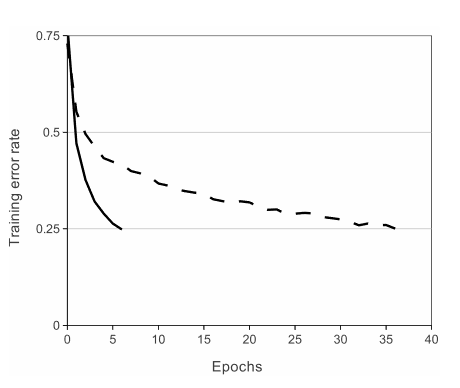
\includegraphics[width=\linewidth]{img/fig8.png}
    \caption{Evolution du taux d'erreur en fonction du cycle sur le dataset CIFAR-10, Trait continue: CNN à 4 couches avec ReLUs, trait discontinue: réseau équivalent avec tanh}
    \label{fig:L8}
\end{figure}
Comme vous pouvez le voir sur ce schéma, en utilisant les ReLUs, nous atteingnons les 25\% taux d'erreur six fois plus vite que la méthode classique.
\par En dehors de ces 2 couches, les auteurs utilisent aussi une couche de pooling (mise en commun), cela permet de réduire la quantité d'information présente sur l'échantillon et de produire 
une sous échantillon plus petit, cela permet d'améliorer la puissance de calcul, au détriment de la perte d'une partie d'information. \\
Il est interéssant de noter que nos auteurs utilisent un filtre de chevauchement "Overlapping Pooling" plutôt qu'un filtre classique de pooling. 
Dans un processus normal de pooling, l'image est d'abord divisé en grille de dimension zxz, à cela nous fesont passer un filtre de taile s à un pas constant de z , les filtres se croisent jamais. \\
Alors que si vous définissez le pas comme s<z, vous obtenez un parcours de l'image où les les filtres se chevauchent en leur bordure. Les auteurs ont observé alors que le 
risque de surapprentissage est plus basse avec cette méthode.

\par Dans ce modèle, il y a d'abord l'application de 96 matrices de convolution de dimension 11x11x3 avec un pas de 4 pixels. 
\\Puis la seconde couche de convolution utilise 256 matrices de dimension 5x5x48.
\\La troisième couche nécessite 384 matrices de dimension 3x3x256.
\\La quatrième couche nécessite 384 matrices de dimension 3x3x196.
\\Enfin la cinquième couche nécessite 256 matrices de dimension 3x3x192.
\\Finalement, les 3 dernières couche "Fully-connected" sont constitué de 4096 neurones chacun.

\par Cette construction de réseau présente près de 60 millions de paramètre, alors que le dataset ILSVRC ne propose que 1000 classes de résultat. 
Ce qui a pousser les auteurs à chercher une solution face au problème du surapprentissage.\\
Une première solution est d'augmenter le nombre de donnée présenté via des transformation préservant le label de l'image. 
Pour cela, les auteurs ont découpé l'image d'entrée de dimension 256x256 sous plusieurs sous-image de dimension 224x224, cela permet d'augmenter la taille 
du vecteur d'apprenti- ssage par 2048. Il est possible d'alterer l'image de départ avec des bruits géneré aléatoirement via une gaussienne.\\
Enfin la deuxième solution proposé est le "dropout", il consiste à mettre 0 à la sortie des neuronnes de la couche caché avec une probabilité de 0.5.
Sans cette technique, le coût sur le temps d'apprentissage aurait doublé car il faudra alors doubler le nombre de cycle pour avoir des résutats qui converge.

\par A la fin de tous ces couche de convolution, pooling et de dropout, nous obtenons une carte neuronnal sophitiqué où l'interprétation de ces résultat nécessite 
l'emploi des couches entièrement connectéee (fully-connected), ces neuronnes particulières ont une connexion total vers toutes les sorties de la couché prédecédente, 
c'est à ce niveau que les résultats sont traduite pour être humainement compréhensible, dans notre exemple, le résultat est la détermination de la classe qu'appartient 
l'objet présente dans l'image. 

\begin{figure}[H]
    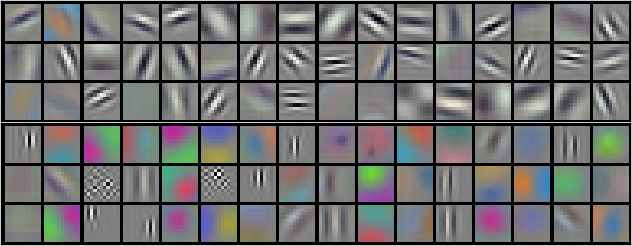
\includegraphics[width=\linewidth]{img/fig10.png}
    \caption{96 convolutional kernels of size 11x11x3 learned by the first convolutionallayer on the 224x224x3 input images. Thetop 48 kernels were learned on GPU 1 whilethe bottom 48 kernels were learned on GPU2}
    \label{fig:L9}
\end{figure}

Comme vous pouvez le voir ci-dessus, le raisonnement machine est assez différente du raisonnement humain, dès la première couche convolution, les matrices résultante n'ont plus 
de propriété spaciale ni sémantique. 

Voici un exemple de résultat de classification pour le dataset ILSVRC-2010.

\begin{figure}[H]
    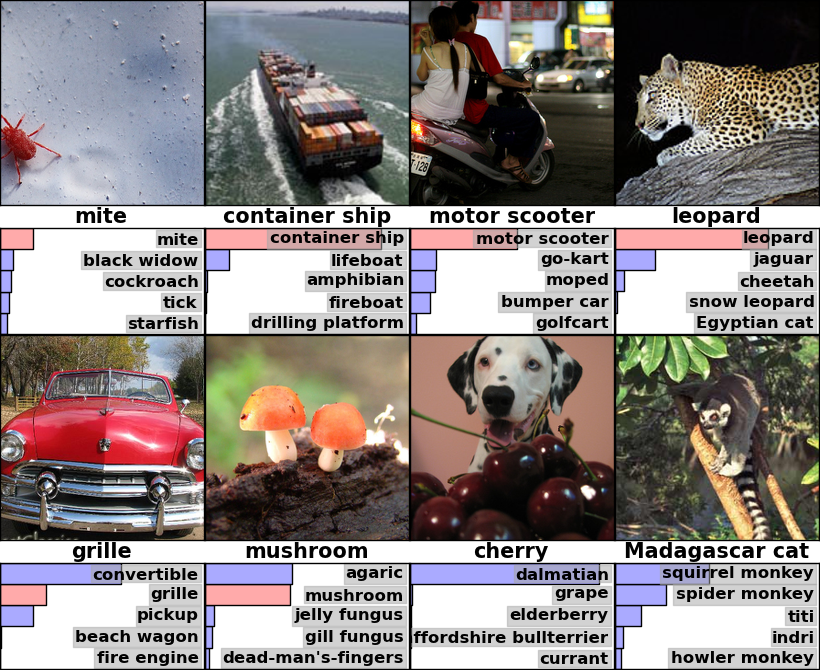
\includegraphics[width=\linewidth]{img/fig11.png}
    \caption{8 ILSVRC-2010 test images and the five labels considered most probable by our model.The correct label is written under each image, and the probability assigned to the correct label is also shownwith a red bar (if it happens to be in the top 5)}
    \label{fig:L10}
\end{figure}

\section{The Elephant in the Room}
\subsection{Présentation des auteurs}
Amir Rosenfeld est un post-doc de l'université de Toronto et de l'université de York.\\
Richard Zemel est professeur au département d'informatique de l'université de Toronto.\\
John K.Tsotos est professeur au département d'ingénieurie electronique et informatique de l'université de Toronto.

\subsection{Présentation de l'article}
Cet article a pour sujet de présenter les familles d'erreur les plus commun dans l'état de l'art des 
detecteur d'objet. La méthode utilisé est la transposition d'image dans une régions de l'image initial.
Cette modification a pour impact des conséquences non local sur la détection de l'objet. \\
Un déplacement positionnel du transplant semble affecter les résultats du détecteur, qui peut modifier l'identité de l'objet détecté.

\subsection{Présentation de l'expérience}
La méthode du détecteur d'objet employé ici est le Faster-RCNN avec un NASNet backbone, en appliquant le programme sur 
une image salon issue du Microsoft COCO object detection benchmark. \\
Les auteurs ont donc littéralement transposé une image d'élephant dans cette image de salon à plusieurs
coordonnées différentes. Ils rélèvent 3 phénomène majeur causé par cette transposition :
\begin{itemize}
    \item La detection est instable, l'object est tout simplement non détecté par le detecteur.
    \item La nature de l'object est incorrect, il est dépendante de la location du transplant.
    \item L'object cause des effets non-locale, les objects qui ne sont pas en chevauchement avec notre transplant peut changer d'identité, boîte de contour ou tout simplement 
        dispaître du champs du detecteur.
\end{itemize}
\begin{figure}[H]
    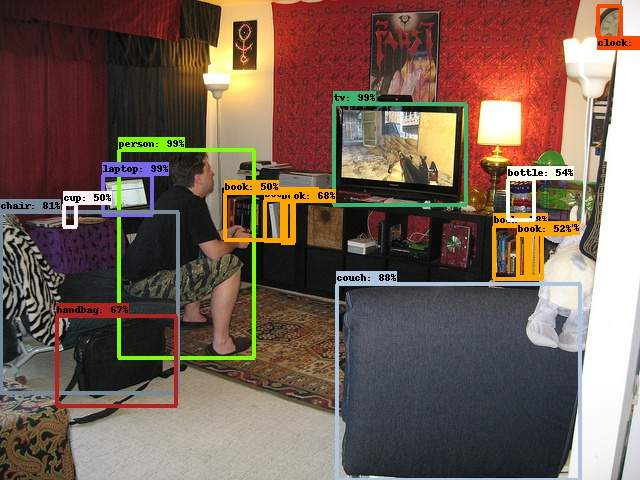
\includegraphics[width=\linewidth]{img/fig12.jpg}
    \caption{Image de départ}
    \label{fig:L11}
\end{figure}

\begin{figure}[H]
    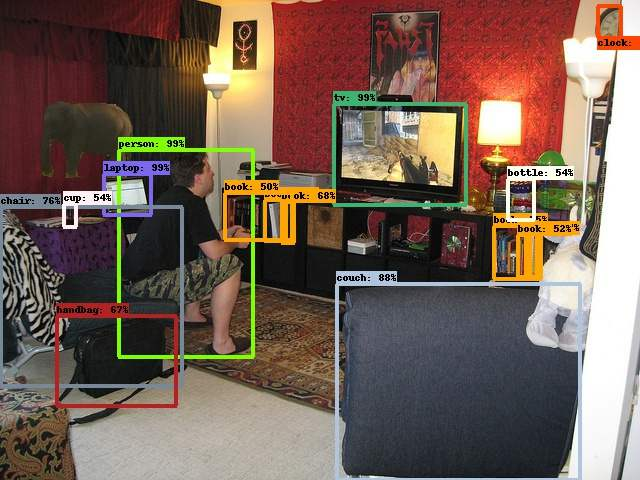
\includegraphics[width=\linewidth]{img/fig13.jpg}
    \caption{Image après transplant de l'éléphant, l'object n'est pas detecté, pas d'incidence sur les autres objects }
    \label{fig:L12}
\end{figure}

\begin{figure}[H]
    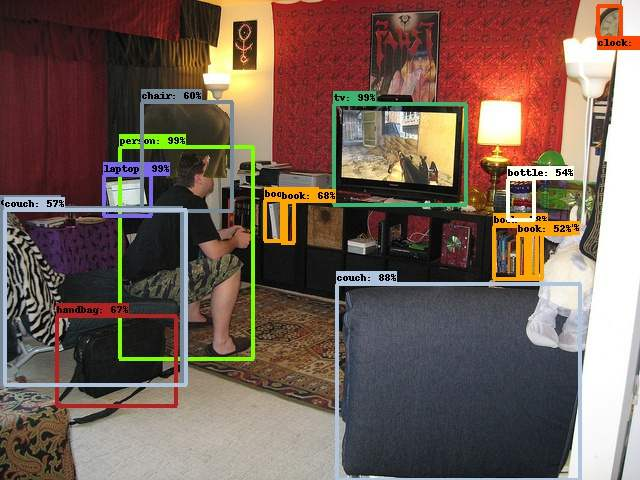
\includegraphics[width=\linewidth]{img/fig14.jpg}
    \caption{L'éléphant est deteté comme un objet "chaise", la tasse n'est plus detecté, l'objet "chair" est devenue "couch"}
    \label{fig:L13}
\end{figure}

\begin{figure}[H]
    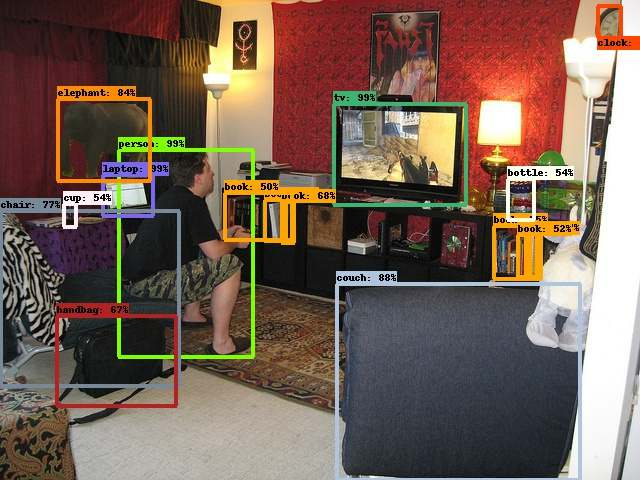
\includegraphics[width=\linewidth]{img/fig15.jpg}
    \caption{L'éléphant est detecté correctemment}
    \label{fig:L14}
\end{figure}

Le résultat est plus impréssionnante si vous essayez du dupliquer certains objets du plan, nous arrivons à des résultats abérrantes.
\begin{figure}[H]
    \centering
    \begin{subfigure}[b]{0.4\linewidth}
      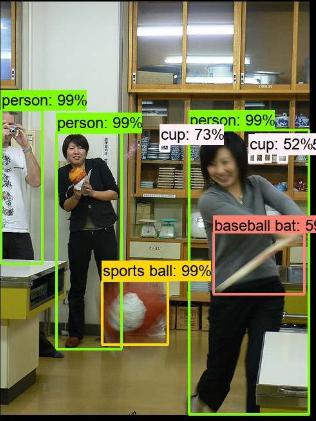
\includegraphics[width=\linewidth]{img/fig17.png}
      \caption{Image initial}
    \end{subfigure}
    \begin{subfigure}[b]{0.4\linewidth}
      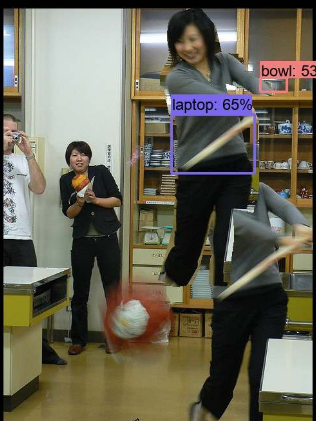
\includegraphics[width=\linewidth]{img/fig18.png}
      \caption{perte de detection}
    \end{subfigure}
    \begin{subfigure}[b]{0.4\linewidth}
        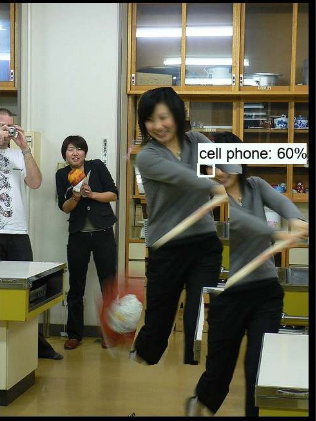
\includegraphics[width=\linewidth]{img/fig19.png}
        \caption{résultat abbérante}
      \end{subfigure}
    \caption{Effets de la duplication}
    \label{fig:L15}
\end{figure}

\subsection{Hypothèses des auteurs}
Les auteurs ont donc proposé quelque hypothèses au vue de ces résultats:
\begin{itemize}
    \item L'occlusion partiel
    \item "Out of Distribution Examples", les transplants peuvent être inconnue du reseau.
    \item Perte de signal à cause des couches de pooling, un sous-échantillonage permet certe un gain en temps d'apprentissage, il y a aussi une perte d'information à ne pas négliger.
    \item Raisonnement contextuel, il est encore rare de voir des classificateur qui intègre la notion d'analyse sémantique, mais nous pouvons voir ailleurs notamment chez les
        les réseaux adverses génératifs.
    \item "Non-Maximal Suppression", qui est une méthode de detection de zone d'interêt peut affecter la décision du programme.
        Par exemple, un objet A qui disparait du detecteur à cause du transplant T peut avoir conséquence de garder l'objet B comme une zone d'interêt alors que B était supprimé dans la version initial à cause de son 
        chevauchement avec A.
    \item "Feature Interference", la zone d'interêt est souvent un rectangle, ce qui fait qu'il ne contient pas seulement l'objet d'interêt, il absorbe aussi les bruits environnante. Du coup l'opération 
    de convolution peut avoir pour conséquence d'inclure les plans derrière l'objet. Dans un autre sens, cela permet d'ajouter une touche d'information contextuel à traîter qui peut être util si nous ne possèdons 
    pas suffisamment d'information sur l'objet due à une occlusion partiel ou à sa faible résolution.
\end{itemize}
\subsection{Critiques de cet article}
L'expérience est intéressante car il souligne certains limites des detecteurs d'objet moderne, cependant il ne propose malheureusement pas de solution à ces problèmes.
Dans un autre sens, est-ce normal qu'un detecteur d'objet doit être capable de detecter certains abbération dont il n'a jamais fait face? 
Il n'y a peut être pas assez d'exemple dans ce sens qui ont été présenté aux neuronnes, parler des résultats sans prendre en compte la nature et la quantité 
de vecteur d'apprentissage n'est pas très convainquant. Le neuronnes a été entrainé par des exemples réel et vous lui présenter des images sémantiquement fausse.\\
C'est bien de se poser la question de pourquoi vous obtenez des résultats abbérante si vous transplanter un éléphant à côté d'un avion qui vole. Mais avez vous déja vue 
un éléphant qui vole à côté d'un avion? \\
Néaumoins, il nous permet de se poser le problématique de quel-est la réaction que nous espérons voir quand une situation comme telle se produisait? 

\section{Conclusion}
Dans le monde de la recherche, il y a deux avis divergeante concernant le CNN, certains pensent qu'il s'agit d'un mirage comme le fut les reseau de neuronne artificiel 
dans les années 1980, d'autres, plus optimiste pensent qu'il s'agit de la dernière révolution dans le domain et que cela va changer radicalement notre 
manière de penser. Personnellement, je suis plutôt optimiste car il existe de plus en plus d'application concret pour les CNN.
L'époque où le monde s'emerveillait devant les performances du CNN à distinguer les chiffres numérique est quand même loin derrière.
De nos jours, le CNN a trouvé des applications passant du simple classificateur d'objet à l'imagerie médicale comme le diagnostique de tumeur.

\section{Remerciements}
Je tiens à remercier Téo Orthlieb pour m'avoir aidé dans mes recherches et qui m'a donné accès aux supports de cours de son Master en informatique à l'université de Montréal. 

\newpage
\printbibliography
\end{document}
